\chapter{Methods}\label{cha:methods}

In this section, I first introduce the fundamental geometric consideration of axisymmetry that applies to each of my methods. I then explain a derivation of paleo- and modern attitude information from sampled locations at the summit of Olympus Mons. I show that paleo-attitude information is incomplete but can be reconstructed uniquely under the axisymmetric assumption given a particular inflation center location. I then explain how to derive the angle of tilt necessary to reconcile the paleo- and modern surface attitudes as a function of distance from the chosen inflation center. By examining the degree to which each inflation center can realistically explain the observed discordance in the region, I determine the most likely inflation centers and test the general validity of the axisymmetric assumption for this system. Once I determine a subset of likely inflation center candidates, I compare the corresponding tilt-distance function with those derived from numerical models of reservoir pressure change. Through the complimentary approaches of mapping and modelling, I evaluate the most likely combinations of reservoir location (laterally by mapping and vertically my modelling) size, and pressure change responsible for observed discordance. 

\section{Axisymmetry}

Numerical models are widely used by physical volcanologists to better understand a wide array of observed phenomena in terms of their underlying mechanisms. One advantage of these simulated models (as opposed to physical models involving real materials) is the diversity of conditions available to be tested, from the deep mantle \parencite[e.g.,][]{redmond_numerical_2004,ogawa_four-stage_2021} or volcanic edifices and their surroundings \parencite[e.g.,][]{isherwood_volcanic_2013} to individual magma reservoirs \parencite[e.g.,][]{grosfils_magma_2007,grosfils_elastic_2015}. Many of these models are axisymmetric, reflecting the common characteristic that many volcanic and magmatic features are roughly circular in plan view. While this sacrifice the ability to assess certain asymmetric features, they are much easier to construct, take much less time to run due to the massively simplified geometry, and often capture major characteristics of the system in question.

\begin{figure}
    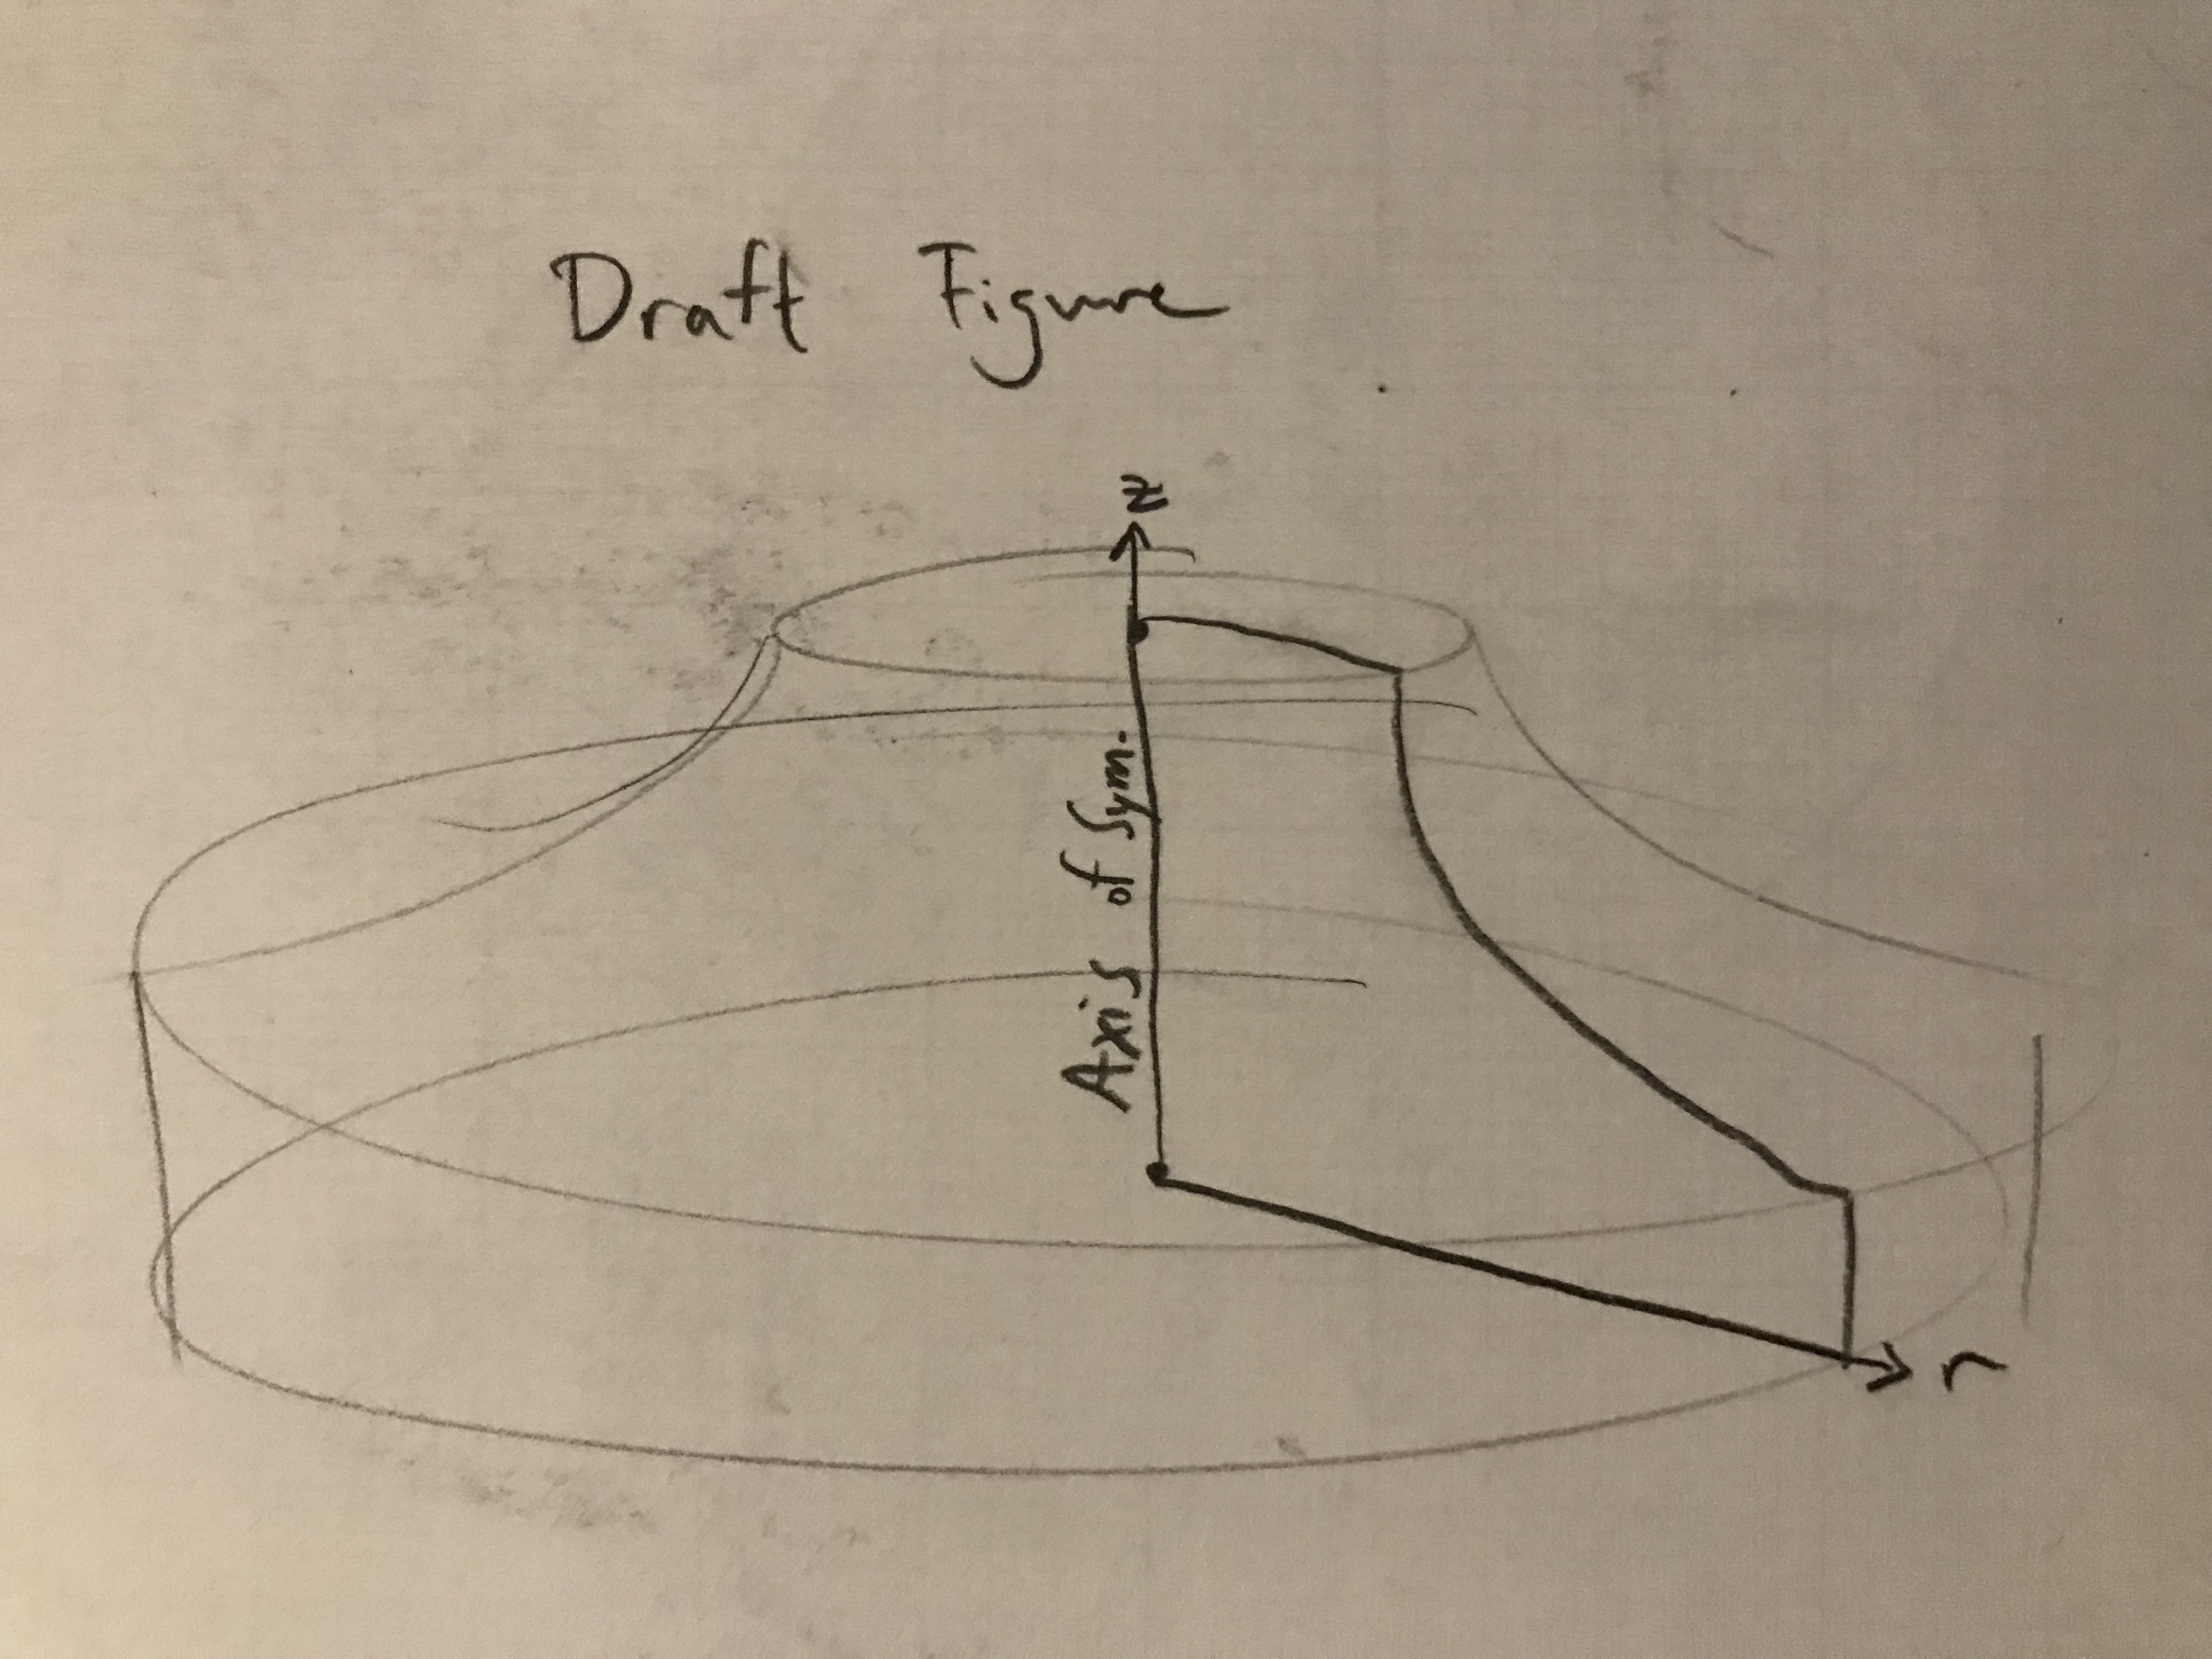
\includegraphics[width=\textwidth]{axisymmetry.jpeg}%
    \caption[Axisymmetric model geometry]{A rotationally symmetric 3D feature is modelled by a single representative cross section.}%
    \label{fig:axisymmetry}
\end{figure}    

In this thesis, I seek to compare surface tilt inferred at the summit with tilt resulting from pressure changes in an underlying magma reservoir. Since this thesis is an early component of a larger research program to assess late Amazonian magmatism at Olympus Mons, I use the simplified\footnote{I justify additional simplifying assumptions in Section~\ref{sec:modelling}.} axisymmetric condition in my numerical models. Therefore, I make the same assumption when estimating tilt from discordant lava flows at the summit.

\section{Mapping}\label{sec:mapping}
\subsection{Preparation of Published Data}

The \acf{CTX}\footnote{aboard the \ac{MRO} spacecraft launched in 2005 by \acs{NASA}.} captures \qty{\sim30}{\km} swaths across the entire martian surface in visible $(\lambda=\qtyrange{500}{800}{\nm})$ greyscale at \qty{\sim6}{\m} spatial resolution. \textcite{Dickson2018AGB} blended these swaths to produce a raster mosaic product (hereafter, ``\ac{CTX} mosaic'') which I use to visually identify and map lava flows and flow channels.

The \acf{MOLA}\footnote{aboard the now-retired \ac{MGS} spacecraft launched in 1996 by \acs{NASA}.} returned topography data with horizontal resolution of \qtyproduct{300 x 1000}{\m} at the equator (better at high latitudes) and elevation uncertainty of \qty{\sim3}{\m}~\parencite{smith_mars_2001}. To improve spatial resolution, additional elevation data from the \ac{HRSC}\footnote{aboard the \ac{MEX} spacecraft launched in 2003 by the \ac{ESA}} was blended to product a \ac{DEM} with \qty{200}{\m} pixel resolution. Each pixel's vertical uncertainty is \qty{\sim1}{\m}, with an additional global uncertainty of \qty{\sim1.8}{\m} in the martian areoid (martian equivalent of Earth's geoid). In this project, the global areoid uncertainty is not a concern because only one region (the summit of Olympus Mons) is considered.

I load these two data sources in an equal-area sinusoidal Mars projection in ArcGIS Pro. The study area is defined by a square \qtyproduct{200 x 200}{\km} centered at the centroid of the outermost \qty{19}{\km} contour,\footnote{This is the highest integer \unit{km} which is roughly circular and completely encloses the caldera complex, implying that it largely records the conical shape of the shield edifice without influence from subsequent caldera collapse or reservoir inflation.} as seen in Figure~\ref{fig:summit}.

\subsection{Study Area Definition \& Preliminary Analysis}

Figure~\ref{fig:summit} shows important topographic patterns at the summit of Olympus Mons. More than \qty{50}{\km} from the center of the figure, topographic contours (\qtyrange{12}{19}{\km}) are fairly regular concentric rings. Closer to the caldera, this axisymmetry breaks down: the caldera complex itself consists of six intersecting collapse pits. On the southern flank, we see a prominent arcuate \qty{20}{\km} contour with the topographic summit (within the \qty{21}{\km} contour) over \qty{20}{\km} from the southern caldera rim. Thus, my first task is to determine the degree to which axisymmetric inflation can apply to an edifice which is not entirely axisymmetric. It is important to point out, however, that the asymmetry inherent to the region is crucial for the discordant flow method to function, as I describe in subsequent sections. 

%\subsection{Proto-Edifice Reconstruction}
% Therefore, I present a reconstruction of the proto-edifice which interpolates the topography of the distal (beyond outer \qty{19}{\km} contour) regions within the central region. This reconstruction is shown in Figure~(NUMBER). This provides an independent estimation of proto-topography to compare with the estimates based on lava flow misalignment.

\subsection{Mapping Lava Features}

I use the \ac{CTX} mosaic to visually identify lava flows near the summit of Olympus Mons. Following \textcite{mouginis-mark_geologic_2021}, I map lobate flow outlines as polygons where possible. From these polygons, I derive centerline features using the \hlss{Polygon To Centerline} tool, as shown in Figure~\ref{fig:flow}.

Where flow margins are not visible, I map channels directly as linear features. I include discontinuous regions where I infer partial collapse of lava tubes yielding skylight chains,\footnote{The assumption of underlying continuity follows, e.g., \textcite{bleacher_olympus_2007,carr_geologic_2010,peters_lava_2021}.} as shown in Figure~\ref{fig:channel}.

\subsection{Paleo-Azimuth from Mapped Features}

% \subsubsection{Segmentation}
% [INCOMPLETE] Bounding box, aspect ratio

I use the \hlss{Calculate Geometry Attributes} tool to find the azimuthal orientation from the start to the end of each feature. This angle is the variable \ac{az1} to each feature, although the following section discussion explains why this variable is not quite ready for use in attitude analysis. While I maintain a consistent ``sense'' in my channel mapping (pointing away from rather than toward the caldera center), the \hlss{Polygon To Centerline} tool does not. Therefore, some flow centerlines need to be reversed using the \hlss{Flip Line} tool.

To determine which centerlines must be reversed, I use the \hlss{Near} tool to determine the azimuth angle from each linear feature to the center of the study area \acs{center}. Here, I leverage my initial observation that all flows in the study area point generally \emph{away} from the caldera center. Therefore, a correctly oriented feature is one where \acs{az1} is \ang{\sim180} away from the calculated angle; at the very least, it should be \ang{90} away. Therefore I select features where this angular difference is less than \ang{90} to reverse using \hlss{Flip Line}, as shown in Figure~\ref{fig:flip-line}. With all features now correctly oriented away from the caldera center, I recalculate the true \ac{az1} value using \hlss{Calculate Geometry Attributes}.

\begin{figure}
    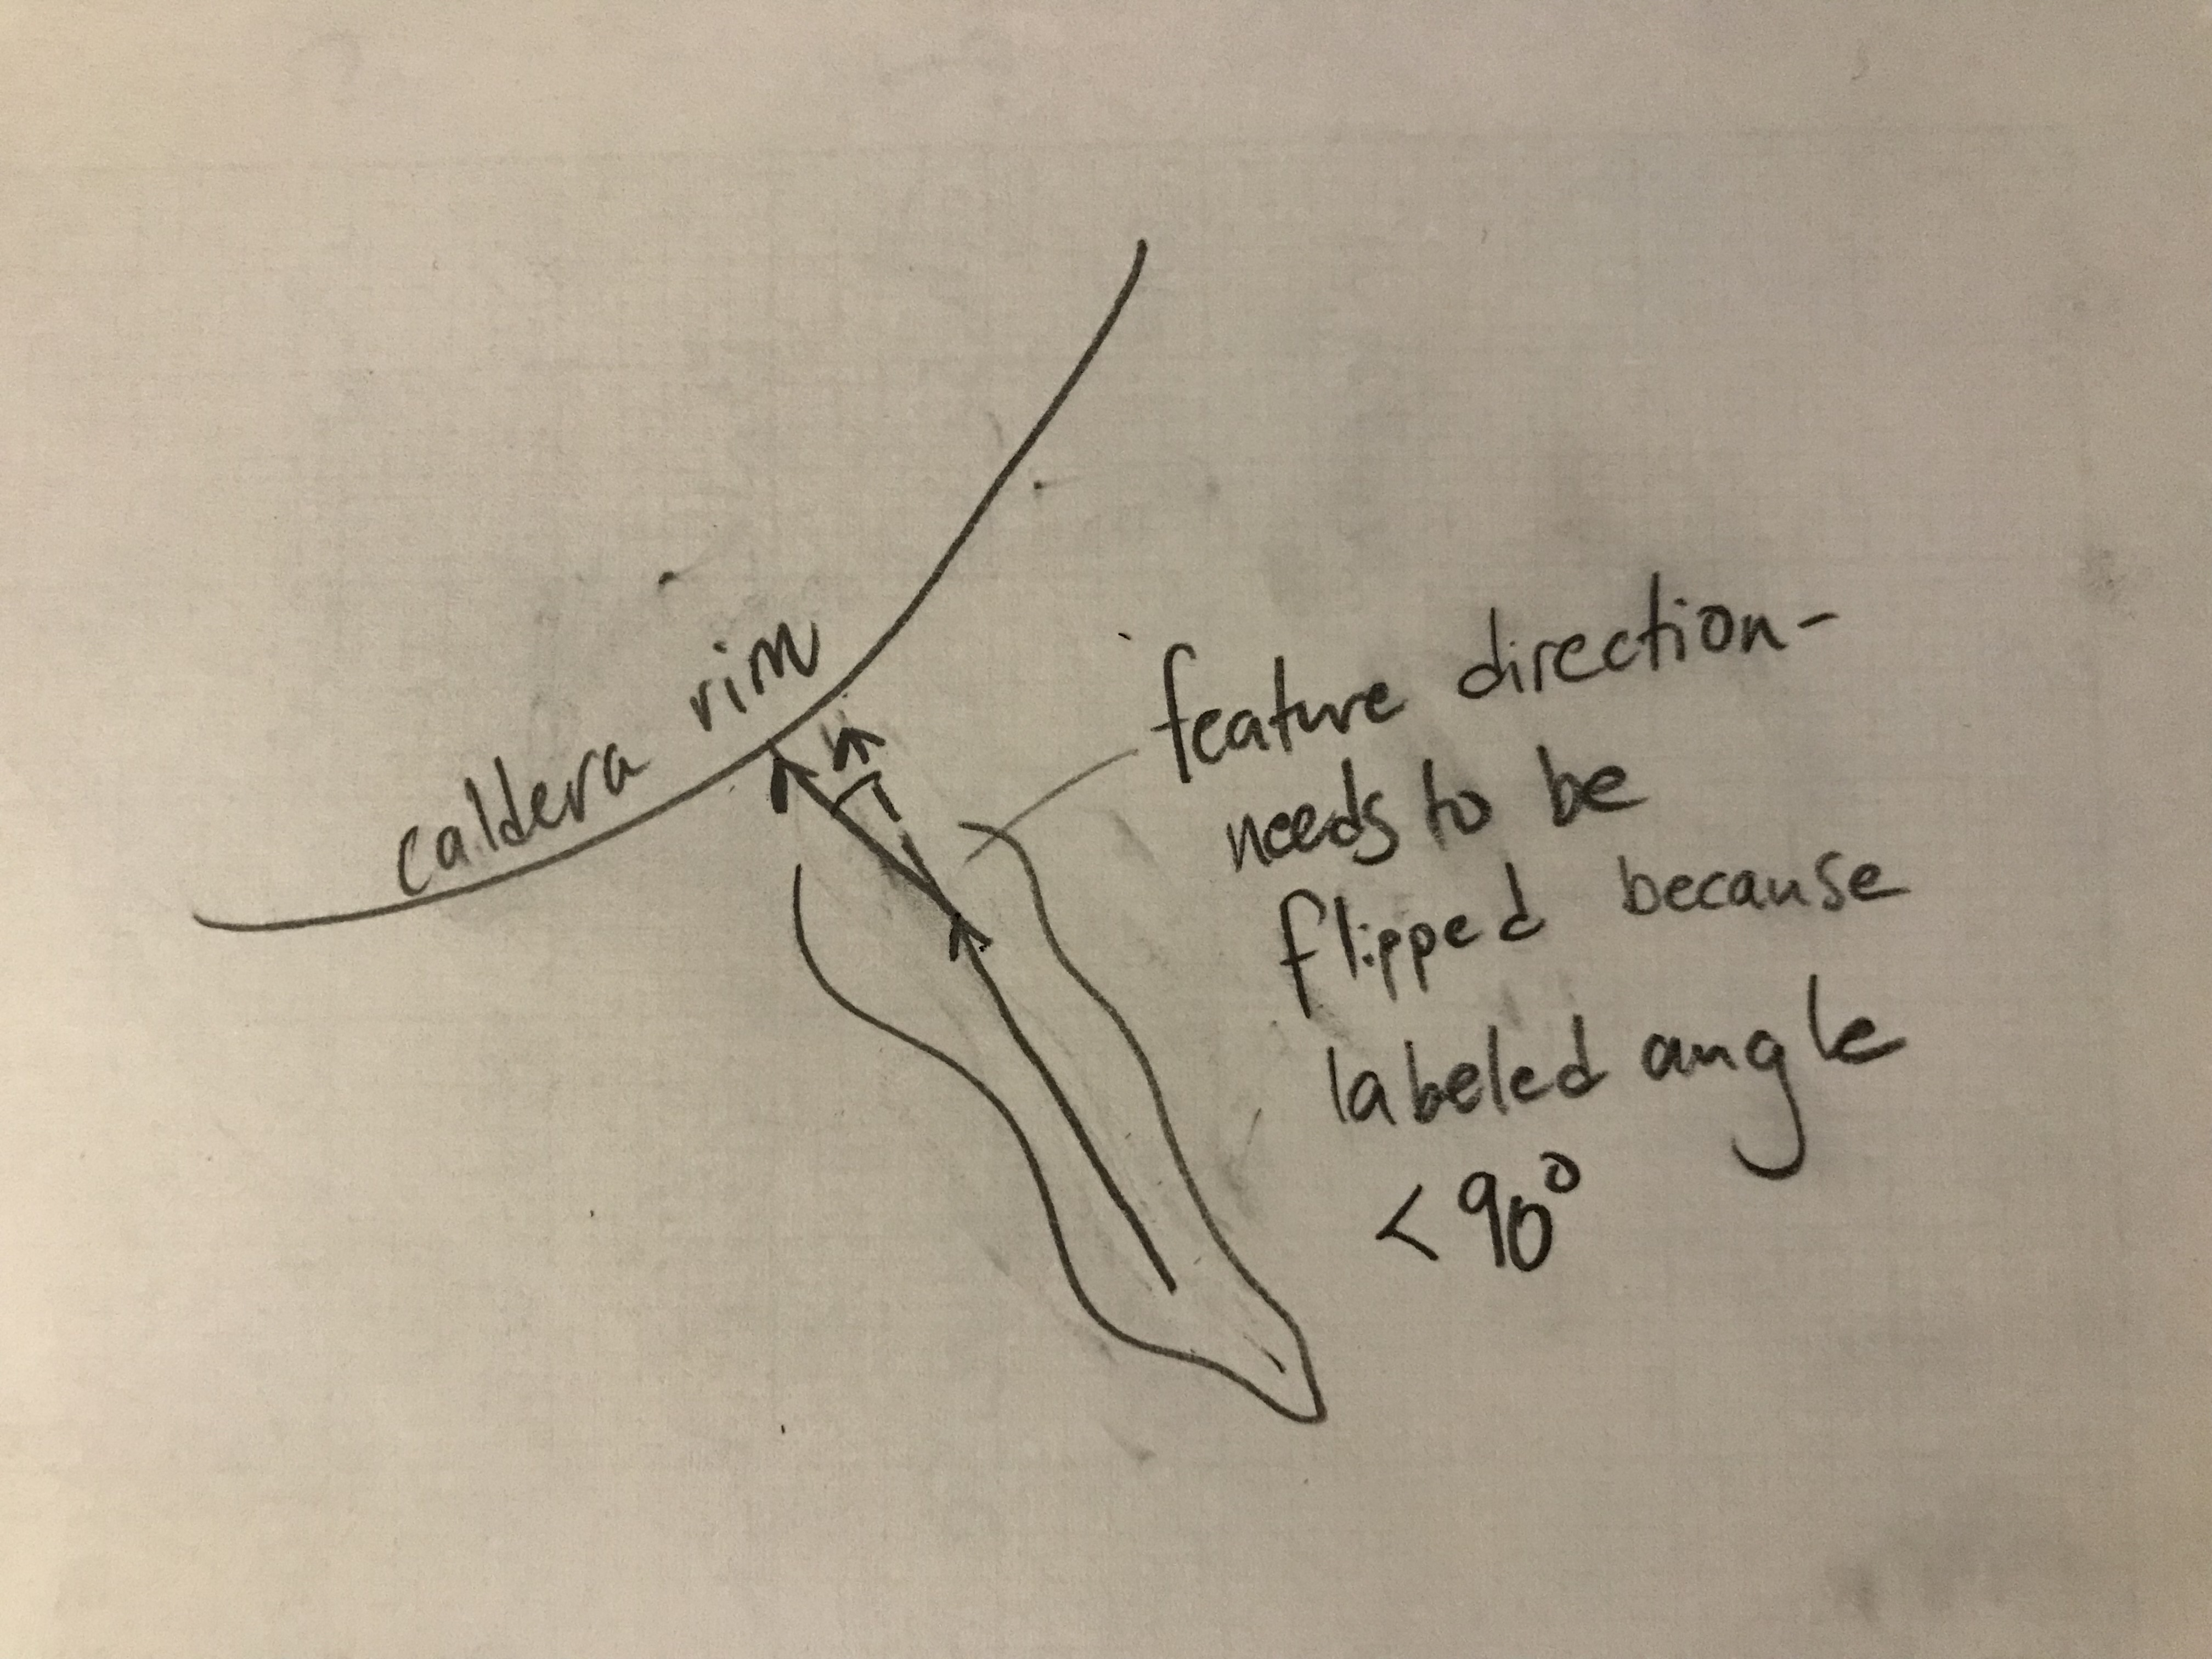
\includegraphics[width=\textwidth]{flip-line.jpeg}%
    \caption{Clip Line}%
    \label{fig:flip-line}
\end{figure}

\subsection{Modern Attitude from Topography}

\newcommand{\samplinginterval}{\qty{3}{\km}}

Along each linear feature, I use the \hlss{Generate Points Along Line} tool sampling interval \samplinginterval\ to create a series of point features where further attitude data collection and analysis will take place. Note that features with length $<\samplinginterval$ are not sampled at all.

\begin{figure}
    \centering
    \begin{subfigure}{\textwidth}
        \centering
        \includegraphics[width=\textwidth]{flow.pdf}
        \caption[Mapped lava flow \& centerline]{A flow with lobate boundaries at each margin is mapped as a polygon (white) from which a linear centerline is derived for sampling.}%
        \label{fig:flow}
    \end{subfigure}
    \begin{subfigure}{\textwidth}
        \centering
        \includegraphics[width=\textwidth]{channel.pdf}
        \caption[Mapped lava channel]{A lava channel is mapped as a linear feature, including regions of discontinuity which are inferred to be collapsed skylight chains over lava tubes.}%
        \label{fig:channel}
    \end{subfigure}
    \caption{Mapping linear features}%
    \label{fig:mapping-linear}
\end{figure}

\begin{figure}
    \centering
    \includegraphics[width=\textwidth]{sampling.pdf}
    \caption[Sampling site selection]{Each linear feature is assigned an average paleo-dip direction. Points are selected for sampling and calculations at \qty{5}{\km} and \qty{3}{\km} intervals for flows and channels, respectively. Paleo-dip direction is assigned to each point from its corresponding line; modern dip and dip direction is assigned to each point from its unique \ac{DEM} neighborhood.}%
    \label{fig:sampling}
\end{figure}

\newcommand{\neighborhood}{\qty{2}{\km}}

The first variable collected is \ac{az1}, which each point inherits from its parent linear feature.

Then, I use the \hlss{Surface Parameters} tool on the \ac{MOLA} \ac{DEM} to compute average topographic \hlss{Slope} and \hlss{Aspect} (downhill azimuth) rasters across the entire study area. To avoid capturing local topographic anomalies, these values are averaged over a ``neighborhood'' with radius \neighborhood. I use the \hlss{Extract Multi Values to Points} tool to assign \ac{sl2} and \ac{az2} to each based on the value of the corresponding raster value at that location. Figure~\ref{fig:tilt-from-map} includes a geometric view of these variables in attitude space alongside \acs{az1}.

% \begin{figure}
%     \floatbox[{\capbeside\thisfloatsetup{floatwidth=sidefil,capbesideposition={left,bottom},capbesidewidth=.55\linewidth}}]{figure}
%     {\caption[Pole to plane $\acs{normal2}=(\acs{az2},\acs{sl2})$]{The attitude of a tilted surface (green) is defined relative to horizontal (grey) by \ac{az2} and \ac{sl2}. \acs{az2} and \acs{sl2} are also the spherical coordinates of a unique unit vector \acs{normal2} which is normal (perpendicular) to the surface. In the subsequent sections, $\acs{normal2}=(\acs{az2},\acs{sl2})$ represents the observed attitude at a sampled location, while $\acs{normal1}=(\acs{az1},\acs{sl1})$ represents the \emph{inferred} paleo-attitude of the same point when the lava flow was emplaced. Azimuth angles increase clockwise from \acf{north} as shown, following geographic convention.}\label{fig:surface}}
%     {\begin{tikzpicture}[scale=4.4,tdplot_main_coords]

% origin
\coordinate (O) at (0,0,0);

% also defines (Pxy), (Pxz), (Pyz), etc.
\tdplotsetcoord{P}{\radius}{\ze}{\az}

% fill flat surface
\fill[color = gray!10!white] (0,0) circle (0.5*\radius);

% define tilted surface
\tdplotsetrotatedcoords{\az}{\ze}{0}

% fill tilted surface
\fill[tdplot_rotated_coords, color = green!40!black, opacity=0.4] (0,0) circle (0.4*\radius);

% downhill line
\draw[arrow, tdplot_rotated_coords] (0,0) -- (0:0.4*\radius);

% horizontal surface (front right)
\fill[color = gray!10!white, opacity=0.6] (\az:0.5*\radius) arc (\az:\az+90:0.5*\radius) -- (0,0);

% perpendicular corners
\draw[tdplot_rotated_coords] (0.25,0,0) -- (0.25,0,0.25) -- (0,0,0.25) -- (0,-0.25,0.25) -- (0,-0.25,0);

% horizontal surface (front left)
\fill[color = gray!10!white, opacity=0.6] (\az-90:0.5*\radius) arc (\az-90:\az:0.5*\radius) -- (0,0);

% z axis
\draw[axis] (O) -- (0,0,0.5*\axislength) node[anchor=south]{$z$};

% line az surface
\draw[very thin, dashed,green!40!black] (P) -- (Pxy) -- (O);
\draw[arrow, green!40!black] (O) -- (P) node[anchor = south west] {\acs{normal2}};

% north axis
\draw[axis] (O) -- (0,0.4*\axislength,0) node[anchor=west]{\acs{north}};

% az angle label
\tdplotdrawarc{(O)}{0.4*\radius}{\az}{90}{coordinate, pin={[pin edge={black},-]-60:\acs{az2}}}{}

% az surface
\tdplotsetthetaplanecoords{\az}

% ze angle label
\tdplotdrawarc[tdplot_rotated_coords]{(O)}{0.4*\radius}{0}{\ze}{coordinate, pin={[pin edge={black},-]80:\acs{sl2}}}{}

% ze angle label
\tdplotdrawarc[tdplot_rotated_coords]{(O)}{0.4*\radius}{90}{90+\ze}{coordinate, pin={[pin edge={black},-]180:\acs{sl2}}}{}

\fill[black] (O) circle (0.2pt);

\end{tikzpicture}}
% \end{figure}

\subsection{Paleo-Slope Calculation}

\begin{figure}
\begin{center}
    \begin{tikzpicture}[scale=5,tdplot_main_coords]
    % origin
    \coordinate (orig) at (0,0,0);
    
    % also defines (Pxy), (Pxz), (Pyz), etc.
    \tdplotsetcoord{P}{\radius}{\ze}{\az}
    \tdplotsetcoord{C}{-0.4*\axislength}{90}{\THETA}
    \tdplotsetcoord{P'}{\radius}{\zen}{\azi}
    \tdplotsetcoord{tiltintercept}{\deltalength}{90}{\THETA-90}
    \tdplotsetcoord{rintercept}{0.68}{90}{\THETA}
    
    % gray rectangle
    \fill[tdplot_main_coords, color = gray!30!white] (orig) -- (tiltintercept) -- (Pxy) -- (rintercept);
    \draw[tdplot_main_coords] (\THETA-90:\radius) arc (\THETA-90:\THETA:\radius);

    % z-axis
    \draw[arrow] (orig) -- (0,0,\axislength) node[anchor=south]{$z$};
    \draw[arrow] (orig) -- (\THETA:\axislength) node[anchor=north east]{$r$};
    \draw[arrow] (orig) -- node[sloped, fill=white, pos=.65]{Tilt Axis} (\THETA-90:\axislength);

    % az' surface
    \tdplotsetthetaplanecoords{\azi}

    \draw[tdplot_rotated_coords] (90:\radius) -- (0,0.76604444*\radius) -- (0,0);
    \tdplotdrawarc[tdplot_rotated_coords, line width = 1mm]{(orig)}{\radius}{0}{90}{anchor=east}{\acs{az1}}

    % \draw[very thin, dashed] (P') -- (P'xy) -- (orig);
    % \draw (orig) -- (P');

    % surface vertical from axis
    \tdplotsetthetaplanecoords{\THETA+90}

    % proj1 line
    \tdplotdrawarc[tdplot_rotated_coords]{(orig)}{\radius}{-90}{0}{}{}
    
    % r-z surface, fill, line
    \tdplotsetthetaplanecoords{\THETA}
    \fill[tdplot_rotated_coords, color = red, opacity = 0.1] (\zenproj:\radius) arc (\zenproj:\zeproj:\radius) -- (0,0);     
    \tdplotdrawarc[arrow, tdplot_rotated_coords]{(orig)}{\radius}{0}{90}{}{}
    \tdplotdrawarc[arrow, tdplot_rotated_coords,red,line width=1mm]{(orig)}{\radius}{\zenproj}{\zeproj}{anchor=south west}{\acs{tilt}}

    % az2 surface
    \tdplotsetthetaplanecoords{\az}
    \draw[very thin, dashed] (P) -- (Pxy) -- (orig);
    % \draw (orig) -- (P);
    
    % az angle labels
    %\tdplotdrawarc{(orig)}{0.33}{\THETA}{\azi}{}{}%{fill=white, anchor=south east}{\acs{beta1}}
    %\tdplotdrawarc{(orig)}{0.37}{\THETA}{\az}{}{}%{anchor=north west}{\acs{beta2}}

    % translate THETA surface to small circle
    \tdplotsetthetaplanecoords{\THETA}
    \tdplotsetrotatedcoordsorigin{(tiltintercept)}
    \draw[tdplot_rotated_coords] (0:\smallcircleradius) arc (0:90:\smallcircleradius) -- (0,0.76604444*\smallcircleradius) -- (0,0) -- cycle;
    \tdplotdrawarc[arrow, tdplot_rotated_coords]{(tiltintercept)}{\smallcircleradius}{\zenproj}{\zeproj}{coordinate}{}
    
    % translate THETA surface to back to great circle
    \tdplotsetrotatedcoordsorigin{(orig)}

    % proj1 plane, line, fill
    \tdplotsetrotatedcoords{\THETA}{-90+\zenproj}{0}
    \tdplotdrawarc[tdplot_rotated_coords, blue, ultra thick]{(0,0,0)}{\radius}{\asindelta}{0}{}{}
    \fill[tdplot_rotated_coords, color = blue, opacity = 0.2] (\asindelta:\radius) arc (\asindelta:0:\radius) -- (0,0) -- (tiltintercept);

    % proj2 plane, fill, line,
    \tdplotsetrotatedcoords{\THETA}{-90+\zeproj}{0}
    \fill[tdplot_rotated_coords, color = green!70!black, opacity = 0.3] (\asindelta:\radius) arc (\asindelta:0:\radius) -- (0,0) -- (tiltintercept);
    \tdplotdrawarc[tdplot_rotated_coords, green!70!black, ultra thick]{(0,0,0)}{\radius}{\asindelta}{0}{}{}
    
    % (az2, sl2) point
    \fill (P) circle (0.2mm) node[anchor = north east] {$(\acs{az2},\acs{sl2})$};
    % \node[right=of P] (P) circle (0.2mm) node[anchor = west] {$(\acs{az2},\acs{sl2})$};
\end{tikzpicture}%%
    \hspace{1cm}%
    \newcommand{\dotradius}{.3pt}%
\begin{tikzpicture}[scale=8]
    \coordinate (orig) at (0,0);

    \coordinate (tiltintercept) at (\deltalength,0);
    \coordinate (pole1) at (\deltalength,\poleoneflatx);
    \coordinate (pole2) at (\deltalength,\poletwoflatx);
    \coordinate (rendpoint) at (0,\poletwoflatx+0.2);
    \coordinate (rintercept2) at (0,\poletwoflatx);    
    \coordinate (rintercept1) at (0,\poleoneflatx);    

    \coordinate (tiltaxisendpoint) at (\deltalength,0);
    
    \draw[dashed] (rintercept2) -- node[fill=white] {$\delta$} (pole2);
    \draw[dashed] (rintercept1) -- (pole1);
    
    % az2, sl2 point
    \fill (pole2) circle (\dotradius);
    \draw[dashed] (orig) -- node[pos=0.6,sloped,fill=white]{$\sin\acs{sl2}$} (pole2);
    \draw (70.5:.25) arc (70.5:90:.25);
    \path (80:.32) node{\acs{beta2}};
    \draw[arrow] (orig) -- (rendpoint) node[anchor=south] {$r$};
    \draw[arrow] (orig) -- node[fill=white] {Tilt Axis}(tiltaxisendpoint);
    \draw (tiltaxisendpoint) -- (pole2);

    % colored great circle segments
    % first radius should be the value of \radius
    \begin{scope}
        \clip (tiltintercept) rectangle (rendpoint);
        \draw[blue, very thick] (\radius,0) arc(0:90:1.3 and 0.425);
        \draw[green!70!black, very thick] (\radius,0) arc(0:90:1.3 and 1.075);
    \end{scope}
    \draw[red, arrow] (0,.425) -- (0,1.075);
    
    % az1 line
    \path (68:.15cm) node[fill=white]{\acs{beta1}};
    \draw (45:.2) arc (45:90:.2);
    % \draw[arrow] (orig) -- (45:\stereoradius) node[anchor=south west] {\acs{az1}};
    \draw[ultra thick,-latex] (orig) -- node[fill=white,sloped,pos=.65] {$\sin\acs{sl1}$} (pole1);

    \fill (pole2) circle (\dotradius);
\end{tikzpicture}%%
    \caption[\Acl{tilt} from mapping]{\textbf{Left:} A quadrant of an upper hemisphere representing attitude space for a sampled point relative to a particular inflation center. The pole labeled $\left(\acs{az2},\acs{sl2}\right)$ represents the modern surface. The line of poles labeled \acs{az1} represents the family of possible paleo-surfaces with downhill direction given by the lava flow direction. The $r-$axis points in the azimuthal direction away from a modelled inflation center \acs{center}. The assumption of axisymmetry imposes a horizontal axis of tilt perpendicular to the $r-$axis. The red arrow labeled \acs{tilt} answers the question: how much tilt \emph{about this axis} bring some pole on line \acs{az1} to pole $\left(\acs{az2},\acs{sl2}\right)$? \textbf{Right:} Plan view of the stereographic projection labeled with important angles for the tilt calculation. Corresponds to horizontal grey rectangle on the left.}%
    \label{fig:tilt-from-map}%
\end{center}
\end{figure}
While the modern topographic surface attitude is fully characterized by \acs{az2} and \acs{sl2}, only the \acf{az1} can be inferred directly from mapped surface features. The axisymmetric model imposes a circumferential tilt axis, that is, modelled tilt is always directly toward or away from the inflation center. I denote the direction away from the inflation center by \acs{bearing}. Figure~\ref{fig:tilt-from-map} illustrates my method for calculating \acf{sl1} under this assumption. The horizontal segment labeled $\delta$ can be defined in two ways:
\begin{equation*}
    \delta = \sin\acs{beta1}\sin\acs{sl1} = \sin\acs{beta2}\sin\acs{sl2},
\end{equation*}
where $\acs{beta1} = \acl{beta1}$ and $\acs{beta2} = \acl{beta2}$. Thus,
\begin{equation}
    \acs{sl1} = \arcsin\left(\frac{\sin\acs{beta2}\sin\acs{sl2}}{\sin\acs{beta1}}\right).\label{eq:sl1}
\end{equation}
\subsubsection{Error Handling}
The computed results from Equation~\eqref{eq:sl1} allow me to handle some issues inherent to the geometry of the problem. First, for some combinations of surface characteristics and center point choice, it is impossible to tilt the once-downhill lava flow about the imposed axis and reach the observed surface attitude. In Figure~\ref{fig:tilt-from-map} a single quadrant contains both $\left(\acs{az2},\acs{sl2}\right)$ and \acs{az1}, but if these fall on opposing sides of the \acs{bearing} line (one on the left, one on the right) there will be no possible vertical translation between the two. Mathematically, this case will arise as a negative value for \acs{sl1}, which is unphysical and must therefore be removed from the subsequent analysis. When a large fraction of sampled points are subject to this error, it signals that the chosen axisymmetric inflation center is inaccurate.

Another problem occurs even in the single-handed (both left or both right) case when:
\begin{equation}
     |\sin\acs{beta2}\sin\acs{sl2}| > |\sin\acs{beta1}|,\label{eq:domain-error}
\end{equation}
because the resulting argument in Equation~\eqref{eq:sl1} is outside the domain of the arcsin function. Physically this case occurs when the lava flow is close to parallel to the radial direction for the modelled inflation center. Additionally, when $|\sin\acs{beta1}|$ is only slightly greater than $|\sin\acs{beta2}\sin\acs{sl2}|$, the calculated \acs{sl1} will be unrealistically large. Both of these cases reflect the difficulty of changing the downhill azimuth of a flow by tipping it roughly in the direction it is already pointing. The quantity of these undefined or unrealistic tilt values provide an additional test on the validity of each axisymmetric inflation center.

Once these issues are addressed by removing \hltt{<null>} (domain error) or negative entries, I record the number of invalid samples and proceed using the valid subset.

\subsection{Deriving Tilt from Mapped Samples}
In Figure~\ref{fig:tilt-from-map}, the arrow which translates the \acs{az1} line onto $\left(\acs{az2},\acs{sl2}\right)$ is a segment of a small circle about the tilt axis. To determine the true angle of tilt I translate this small circle onto the corresponding great circle along the blue and green great circle segments, respectively. [NOTE: How could I rephrase this? It's kind of like an apparent dip problem but would it be confusing to mention this?] The difference between these two transformations is the tilt: 
\begin{equation}
    \acs{tilt} = \arctan(\tan\acs{sl2}\cos\acs{beta2}) - \arctan(\tan\acs{sl1}\cos\acs{beta1}).\label{eq:tilt-from-map}
\end{equation}
Unlike Equation~\eqref{eq:sl1}, these calculations will not yield any domain errors. The only regions of high numerical sensitivity are near the poles of the tilt axis, but this occurs only for near-vertical observed surfaces (to yield high values of $\delta$ in Figure~\ref{fig:tilt-from-map}) which is unphysical.

\subsection{Implementation}

To identify the most likely inflation center candidates I use the \hlss{Generate Tesselation} and \hlss{Feature to Point} tools to generate an evenly spaced array of points in the caldera vicinity as shown in Figure [Need to make map here].

Then, I need to compute Equation~\eqref{eq:tilt-from-map} for each sampled point (from flows and channels) and from each inflation center point. Here I use the \hlss{ModelBuilder} tool to:
\begin{enumerate}
    \item Iterate over the feature class shown in Figure~[CENTERS] (perform the subsequent steps in order using a different point each).
    \item Run the \hlss{Near} tool to compute the distance and direction from the single inflation center to the sampled point. The former is necessary for direct comparison with the axisymmetric model results, step is necessary to define \acs{beta1} and \acs{beta2} for each point.
    \item Evaluate Equation~\eqref{eq:sl1} for each point.
    \item In addition to the values which are already \hltt{<null>} due to the domain error in Equation~\eqref{eq:sl1}, I set any negative values to \hltt{<null>}.
    \item Evaluate Equation~\eqref{eq:tilt-from-map} for each valid point.
    \item Export a table with attributes of each sampled point: some of which depend only on the point itself (calculated in Section [Previous]) and some of which depend on the relationship between the sampled point and the inflation center [calculated in this iteration]. With the data exported, the iteration begins again with the next inflation center candidate.
\end{enumerate}
The final product of this process is a collection of \hltt{.csv} files---one for each inflation center candidate---each containing the axisymmetric tilt angle implied at each point. 

% FIGURE of CENTER POINTS

\subsection{Evaluating Inflation Center Candidates}

I evaluate each inflation center point by several criteria derived from this exported data using the Python programming language in a Jupyter Notebook. First, I determine what fraction of the sampled data points are possible to account for mathematically: those not ruled out by the sign error in Equation~\eqref{eq:sl1} and the domain error in Equation~\eqref{eq:domain-error}. Then, I choose a cutoff angle (tentatively, a generous \ang{5}) and rank the output tables by the fraction of calculated tilts whose absolute value is within the cutoff magnitude. 

After evaluating these criteria, I export a table containing each center point with its score on each criterion. I rejoin this table to the original point features to examine the spatial distribution of the most likely inflation centers.

Within these most likely inflation center datasets, I search scatter plots of tilt as a function of distance, looking for qualitative patterns matching the expected pattern (discussed in the following section).

I conduct the analysis outlined above using various subsets of the sample point data to determine whether multiple inflation centers are necessary to explain inflation in different regions. I pay particular attention to the highly discordant flows near the southern summit region shown in Figure~\ref{fig:uphill-flows}.

\section{Modelling}\label{sec:modelling}

\subsection{Preliminary Assumption Testing}
% Gravity - Prestress
% Topography
% Looking to conclude that flat, non-gravitational model is sufficient for tilt to make previous section valid (arbitrary center points)

% Include specific methods and results in Appendix rather than main results
% Maybe move Mogi Model solution to an appendix as well.

\subsubsection{Comparison with Analytical Solution}
The discrete Equation~\eqref{eq:tilt-from-flat-model} can be taken to the continuous limit by dividing each term in the numerator and denominator by the element width \acs{dr1}:
\begin{equation}
\acs{tilt}
    = \lim_{\acs{dr1}\to0} 
    \arctan\left(\dfrac{-\acs{ddisp_z}/\acs{dr1}}{\acs{dr1}/\acs{dr1}
    + \acs{ddisp_r}/\acs{dr1}}\right) = 
    \arctan\left(\dfrac{-\acs{disp_z'}}{1+\acs{disp_r'}}\right),\label{eq:tilt-from-flat-analytical-model}
\end{equation}
where $'$ denotes the derivative with respect to $r_1$. I use the \textcite{mogi_relations_1958} Model:
\begin{gather}
    \acs{disp_z} = ad{(d^2+r^2)}^{-1.5},\label{eq:uz_mogi}\\
    \acs{disp_r} = ar{(d^2+r^2)}^{-1.5},\label{eq:ur_mogi}\\
    a = {3R^3\Delta P}/{4G},\nonumber
\end{gather}
where $R$ is the reservoir radius, $\Delta P$ is the overpressure, and $G$ is the elastic shear modulus. Differentiating Equations~\eqref{eq:uz_mogi} and~\eqref{eq:ur_mogi}, substituting into Equation~\eqref{eq:tilt-from-flat-analytical-model}, and simplifying:
\begin{equation}
    \boxed{\acs{tilt} = \arctan\left(\frac{3adr}{{(d^2+r^2)}^{2.5}+ad^2-2ar^2}\right).}\label{eq:tilt-from-mogi-model}
\end{equation}
I compare this result with the numerical results for equant $(\acs{Rr}=\acs{Rz})$ reservoirs to validate the method.

\subsection{Deriving Tilt from Modelled Displacement}

I use the numerical modelling software COMSOL Multiphysics 6.1 (COMSOL) to construct a numerical representation of Olympus Mons. The model is axisymmetric, about the center point discussed previously as the center of the \qty{19}{\km} contour. A profile from due south of this point is used as the 

The numerical formula for \acf{tilt} given \acs{disp_a} and \acs{disp_b} is derived from Figure~\ref{fig:tilt-from-model}:
\begin{equation}
    \acs{tilt} = \arctan\left({\acs{dz1}}/{\acs{dr1}}\right) - \arctan\left(\dfrac{\acs{dz1}+\acs{ddisp_z}}{\acs{dr1}+\acs{ddisp_r}}\right).\label{eq:tilt-from-model}
\end{equation}
For a flat model ($\acs{dz1} = 0$), Equation~\eqref{eq:tilt-from-model} reduces to
\begin{equation}
    \acs{tilt} = 
    -\arctan\left(\dfrac{\acs{ddisp_z}}{\acs{dr1}+\acs{ddisp_r}}\right).\label{eq:tilt-from-flat-model}
\end{equation}

\begin{figure}
    \newcommand{\uar}{3.5}
\newcommand{\uaz}{11}
\newcommand{\ubr}{5.5}
\newcommand{\ubz}{4.5}
\newcommand{\dz}{2.5}
\newcommand{\dr}{8}

\begin{tikzpicture}[scale=0.95]
    \coordinate (orig) at (0,0);
    \coordinate (A1) at (0,\dz);
    \coordinate (B1) at (\dr,0);
    
    \path (A1) + (\uar, \uaz) coordinate (A2);
    \path (B1) + (\ubr, \ubz) coordinate (B2);

    \path (A1) + (\uar - \ubr, \uaz - \ubz) coordinate (A1_trans);

    \draw[-latex] (orig) --+ (-0.5,0) node[anchor=east] {\acs{center}};

    \draw[] (orig) -- node[fill=white] {\acs{dr1}} (B1);
    \draw[] (orig) -- node[fill=white] {$-\acs{dz1}$} (A1);

    \draw[ultra thick] (A1) -- node[sloped,fill=white] {Original Surface} (B1);

    % % main displacement vectors
    \draw[arrow,gray] (A1) -- node[sloped, fill=white] {\acs{disp_a}} (A2);
    \draw[arrow,gray] (B1) -- node[sloped, fill=white] {\acs{disp_b}} (B2);
    
    % % \fill[blue, opacity = 0.15] (B1) --++ (162.7:2.5) arc (162.7:180:2.5);
    % % \path (B1) + (172:2) node {\acs{proj1}};
    
    \draw[arrow,gray,dashed] (A1) -- node[fill=white] {$-\acs{ddisp}$} (A1_trans);
    
    \draw[arrow,gray,dashed] (A2) --node[fill=white] {$\acs{disp_b}$} (A1_trans);
    
    % % \fill[red, opacity = 0.3] (B2) --++ (138:2.75) arc (138:162.7:2.75);
    % % \path (B2) + (150:2) node {\acs{tilt}};

    % % Draw displaced surface lines
    \draw[ultra thick] (A1_trans) -- node[sloped,fill=white] {Displaced Surface (Translated)} (B1);
    \draw[ultra thick] (A2) -- node[sloped,fill=white] {Displaced Surface} (B2);
    
    % % draw points
    \fill (B1) circle (2pt) node[anchor = north] {$B_1$};
    \fill (A2) circle (2pt) node[anchor = south] {$A_2$};
    \fill (B2) circle (2pt) node[anchor = west] {$B_2$};
    \fill (A1_trans) circle (2pt);
    \fill (A1) circle (2pt) node[anchor = east] {$A_1$};
    
\end{tikzpicture}%
    \caption[\Acl{tilt} from modelling]{Cross-sectional view of a surface element in the axisymmetric model. As in Figure~\ref{fig:tilt-from-map}, the $r-$axis points away from the inflation center. During the model, the two vertices $A_1$ and $B_1$ of a surface element are displaced along \acs{disp_a} and \acs{disp_b} to reach a final position at $A_2$ and $B_2$, respectively. I illustrate the difference $\acs{disp_b} - \acs{disp_a} = \acs{ddisp}$ in terms of its components \acs{ddisp_r} and \acs{ddisp_z}. Notice that $z-$component terms are negative to ensure that tilt away from the inflation center yields a positive tilt \acs{tilt}, as shown in red. To calculate \acs{tilt}, I determine the slopes of segments $\overline{A_1B_1}$ and $\overline{A_2'B_1}$ using the labeled horizontal and vertical segments, convert these slopes to angles, and take their difference.}%
    \label{fig:tilt-from-model}%
\end{figure}

\subsection{Implementation}

As in my mapping implementation, I leverage iteration to conduct a sequence of analyses which are identical except for specifically controlled parameters. I run a series of numerical models using the \hlss{Parameter Sweep} tool over \ac{DtT}, \ac{Rr}, \ac{Rz}, and a \ac{mult}:
\begin{equation}
    \acs{dP}=\acs{mult}\times\acs{rhor}\times\acs{g}\times\acs{DtT},
\end{equation}
where \acs{dP} is the simulated over- (positive) or under-pressure in the reservoir. For each numerical model, I output surface displacement in the radial and vertical direction as a function of distance from the inflation center. Post processing and implementation of Equation~\eqref{eq:tilt-from-model} is explained in the linked Jupyter notebook.